\section{Description of solid breeder blankets}\label{sec:intro-blanket-description}

The solid breeder blanket is an integral part of the power generation and fuel cycle in a fusion reactor. Before describing the specific functional requirements of the solid breeder blanket, we will review the major features of a fusion reactor fuel cycle. The current, worldwide choice for fusion reaction is deuterium-tritium (DT). The choice is based on DT having a high reaction probability at the lowest ion temperature, high energy yield, fuel availability, and reaction products (how harmless are the daughter products). The DT reaction is

\begin{align}
	\mathrm{D} +~\mathrm{T}&\xrightarrow{}~^4\mathrm{He}+\mathrm{n}+17.58~\text{MeV} \label{eq:dt-reaction}
\end{align}

Of the two isotopes fused, deuterium ($D$, or $^2$H) is a stable isotope and is naturally occuring in an average abundance of 0.015 mole percent in water on Earth. But tritium ($T$, or $^3$H), contrarily, is radioactive with a half life of only about 12.32 years; naturally decaying as $\beta^-$ emitter (no $\gamma$ rays),

\begin{align}\label{eq:t-decay}
	\mathrm{T} \xrightarrow{}~^3\mathrm{He} + \beta^-
\end{align}

Owing to its short half life, any naturally occurring tritium decays at such a rapid pace it will never accumulate. Because of this, to use the DT reaction in a fusion power plant, tritium will need to be generated artificially (breeded) and collected as fuel source. 
%~~~~~~~~~~~~~~~~~~~~~~~~~~~~~~~~~~~~~~~~~~~~~~~~



%~~~~~~~~~~~~~~~~~~~~~~~~~~~~~~~~~~~~~~~~~~~~~~~~
\subsection{Tritium breeding}

One way of breeding tritium for a fusion reactor is to include a so-called tritium breeding blanket that surrounds the fusion plasma with some phase of lithium. Natural lithium interacts with the neutrons with the two most common reactions given in Eq.\ref{eq:lithium-t}

\begin{subequations}\label{eq:lithium-t}
\begin{align}
	\mathrm{n}_\text{fast} + ~^7\mathrm{Li} &\xrightarrow ~\mathrm{n}+\alpha + \mathrm{T} -2.47~\text{MeV}\label{eq:li7-t}\\
	\mathrm{n}_\text{thermal} + ~^6\mathrm{Li} &\xrightarrow ~ \alpha + \mathrm{T} +4.78~\text{MeV} \label{eq:li6-t}
\end{align}
\end{subequations}

where we haved used the common short-hand of $\alpha$ in place of the helium nucleus. The cross-sections of the lithium reactions are given in Fig.~\ref{fig:li-xsects}

\begin{figure}
	\centering
	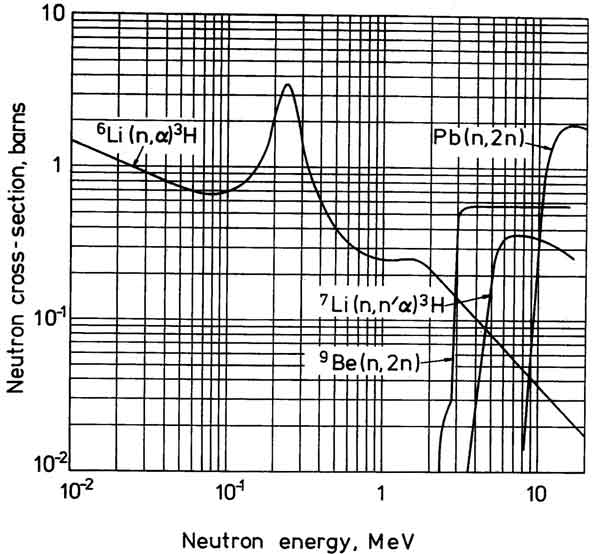
\includegraphics[width=0.8\textwidth]{chapters/figures/breeding_xsecs} 
	\caption{Cross-sections of various blanket materials. Note the threshold for the $^7$Li and neutron multiplying reactions.}
	\label{fig:li-xsects}
\end{figure}

Serendipitously, the DT reaction itself produces a high energy neutron (see Eq.~\ref{eq:dt-reaction}) that can interact with the two isotope reactions of Eq.~\ref{eq:lithium-t}. A commonly used classification of the efficacy of a breeding blanket is through the `tritium breeding ratio', defined as 

\begin{equation}
	\text{TBR} = \cfrac{\dot{N}^+}{\dot{N}^-}
\end{equation}

where $\dot{N}^+$ is the number of tritium atoms generated per unit time in the blanket and $\dot{N}^-$ are the number of tritium atoms consumed per unit time.

For a DT cycle that creates a single neutron we can simplify this definition to say the tritium breeding ratio is the number of tritium atoms produced in the blanket per fusion neutron. If every single neutron from the fusion reaction were to be captured by lithium, we would have a TBR $=1$ and would be ideally self-sufficient. In reality, when we take into account neutron interactions with materials in the structure, tritium retention in material, or losses due to inefficiency in collecting tritium, self-sufficiency of the fuel cycle is not possible unless the fusion neutron is multiplied before interacting with lithium. The extra neutrons allow a TBR$>1$ to be realized and counter-act losses. Materials to act as neutron multipliers would be those that have large neutron multiplication cross sections (over large energy ranges). They react with (n,2n) or (n,3n). Furthermore it is desirable that they have low neutron absorption and that they would have a favorable impact on energy multiplication. 

The two most prominently analyzed neutron multipliers for a fusion reactor are beryllium and lead. Beryllium has a very high nuclide density while also being very light, with a high melting temperature, and high thermal conductivity. However it undergoes a 2-$\alpha$ reaction that causes trapped helium to swell the material. There is also a rarely occurring reaction with beryllium that generates tritium; it is frequent enough to cause a concern with contamination. For solid breeding blankets, beryllium has been pegged as the element of choice. The exact details of implementing a neutron multiplier are beyond the scope of this report.

Clearly it is essential to engineer a device that surrounds the fusion reaction, captures the ejected neutron to breed tritium, and allows recovery of that tritium to attain self-sufficiency. Additionally, the blanket must also be capable of converting energy deposited from neutrons, $\gamma$ rays, and surface radiation from the plasma and then recovering the energy at high tempreatures for efficient power production in the fusion power plant.

Blanket designs have evolved significantly since their introducetion in the 1970s. Some features of current breeder designs will be discussed next.
%~~~~~~~~~~~~~~~~~~~~~~~~~~~~~~~~~~~~~~~~~~~~~~~~



%~~~~~~~~~~~~~~~~~~~~~~~~~~~~~~~~~~~~~~~~~~~~~~~~
\subsection{Solid breeder design}
Pure lithium has a melting temperature of only about \si{180 C} so must be combined with a refractory material if we choose to keep it in solid form at high temperatures. To date, most parties researching solid breeder blankets are focusing on lithium orthosilicate ($\lis$) or lithium metatitanite ($\lit$) as candidate ceramics, though other candidate ceramics do still exist. Lithium oxide had been considered because of its favorable lithium density, among other attractive features, though the reaction of lithium with elemental oxygen is a concern. Pure lithium reacts with oxygen exothermically in reactions such as

\begin{subequations}
\begin{align}
	2\mathrm{Li} + \frac{1}{2}\mathrm{O} &\rightarrow \mathrm{Li}_2\mathrm{O} - 142.75~\text{kCal/mol}\\
	2\mathrm{Li} + \mathrm{O} &\rightarrow \mathrm{Li}_2\mathrm{O}_2 - 151.9~\text{kCal/mol}
\end{align}
\end{subequations}

Of primary concern in lithium fires is the peak flame temperature. This will determine, to a large extent, whether many radioactive species become air-borne by vaporization. The flame temperature depends on many variables. Some investigations found it to be about 2500 K which would cause some materials to melt but not vaporize. [cite Abdou's class notes?]

Large thermal gradients in the solid lithiated ceramics will cause large stresses across large characteristic lengths. Avoiding those stresses has led to most solid breeder designs implementing packed beds of small, spherical (or near-spherical) pebbles. The solid breeder in many current designs for ITER feature sub-module units of packed beds. From the point of view of pebble bed thermomechanics, this has the advantage of producing units individually that can be tested and qualified to desired packing states (and therefore thermomechanics) during the design phase.

The packed bed will be contained by ferritic or austenitic steel that is itself cooled, most commonly, by a high pressure helium gas. A low-pressure (just above atmospheric) purge gas of hydrogen-doped helium 




% 
